\documentclass[12pt,oneside,openany,a4paper,%..... Layout
               afrikaans, english,%.............. Global language selection
               ]{memoir}

 \usepackage[masters-t,%.......................... Master thesis
             goldenblock,%........................ A5 type block (or a5block or wide)
            ]{usthesis}%.......................... US thesis style with memoir

%
% PLEASE read the USthesis documentation for the class options
% and how to set line and paragraph spacing
%

%==== Math setup ====================================================
 \usepackage{amsmath}%............................ Advanced math (before fonts)
 %\usepackage{amssymb}%............................ AMS Symbol fonts

%==== Font setup (default is Computer Modern) =======================
 \usepackage[T1]{fontenc}%........................ Type 1 fonts
 %\usepackage{fourier}
 \usepackage{textcomp}%........................... Additional text character
 \usepackage{bm}%................................. Bold math symbols (after fonts)
 
 %==== Language setup ================================================
 \usepackage[latin1]{inputenc}%................... Recognizes ê, ë, etc
 \usepackage{listings}
 \usepackage{babel}%.............................. Language setup
 \usepackage[colorlinks,urlcolor=blue,breaklinks=true]{hyperref}
 
 \hypersetup{
    colorlinks=true,
    linkcolor=blue,
    filecolor=magenta,      
    urlcolor=cyan,
    pdftitle={MSc:2018-Rust},
    pdfpagemode=FullScreen,
}

\usepackage{multicol}

%==== Ref's, Bib's and Nomencl ======================================
\usepackage[toc]{glossaries}%.......................... List of symbols (in usthesis pack)%
\makeglossaries
%Glossaries Entries HERE ===========================================

\newglossaryentry{autotrophs}{name=Autotrophs,description={Producers of energy, synthesising compounds needed to sustain life from various processes \textit{i.e.} plants, algae and bacteria. For this text the term will be used solely to denote organisms deriving their energy by photosynthetic means}}

\newglossaryentry{bit}{name=BIT,description={Basic unit of computer information. A representational state, \textit{i.e.} binary digits (0,1), boolean operators (true,false), activation states as in on,off, bound vs unbound (enzyme ligand interaction) or more general any two valued attribute}}

\newglossaryentry{$k_b$}{name=Boltzmann Constant,description={Has the dimension of energy divided by temperature, as such this is a constant relating average kinetic energy to temperature:
$k_b=1.38064852\times10^{-23}m^2kgs^{-2}K^{-1}$
}}

\newglossaryentry{api}{name=API,description={Application Program Inferface; As the name suggests is a link between various applications or programs described by a clearly defined API specification}}

\newglossaryentry{sbml}{name=SBML,description={Standard Biological Mark-up Language; A standardized description language used to transcribe biological model data. For more information visit \href{sbml.org}{www.sbml.org}}}

\newglossaryentry{mf}{name=MF,description={Matrix Format; An internal model format used by \href{https://jjj.bio.vu.nl}{JWS Online} metabolic network calculators.  (\textit{i.e.} \href{https://jjj.bio.vu.nl/rest/models/teusink/mf/}{Teusink-Glycolysis.mf})}}

\newglossaryentry{rest}{name=REST,description={Representational State Transfer; A specific subset of \gls{api} allowing for a stateless communication protocol}}

\newglossaryentry{call}{name=call,description={A \gls{request} made to access services or data on a server, remote or local}}

\newglossaryentry{request}{name=request,description={A set of instructions sent to a server, intended to invoke some action or \gls{response}}}

\newglossaryentry{response}{name=response,description={Reply action from server based upon instructions sent via \gls{request}}}

\newglossaryentry{mca}{name=MCA,description={Metabolic Control Analysis; A subset of sensitivity analysis, a mathematical framework used to quantify metabolic, signalling and genetic pathways}}

\newglossaryentry{steady-state}{name=steady-state,description={A state whereby the rate of formation of metabolites equal the rates of degradation, leaving the system in a dynamic equilibrium}}

\newglossaryentry{url}{name=Universal Resource Locator,description={Simply referred to as a web address. a URL represents the location of various web-based resources.}}



\usepackage[square,numbers,sort&compress]{natbib}
\bibliographystyle{abbrvnat}
    \renewcommand\bibfont{\small}

    %% For usmeg-a, the bib is a list of references. If you
    %% are using usmeg-n comment out the following lines
    \addto{\captionsafrikaans}{\renewcommand{\bibname}{Lys van Verwysings}}
    \addto{\captionsenglish}{\renewcommand{\bibname}{List of References}}

%==== Graphics and Color ============================================
\usepackage{graphicx}%........................... Graphicx loaded in usthesis
\graphicspath{ {figs/} }
\usepackage{color}%.............................. Color setup
\usepackage{eso-pic}%............................ Shipout commands for watermark
    \newcommand*{\WaterMark}[2][0.15\paperwidth]{%
        \AddToShipoutPicture*{\AtTextCenter{%
                \parbox[c]{0pt}{\makebox[0pt][c]{%
                    \includegraphics[width=#1]{#2}}}}}}




%==== Local Defs ====================================================
\makeatletter
%
% Please insert user defined commands here
% and NOT in the document itself!
%

\makeatother

%==== TITLE PAGE ====================================================
\title{\bfseries
       \AorE{%-- Afrikaans ------------------------------------------
             'n Rekenaar gedrewe ondersoek in die verwantskap tussen ekwilibrium en fluksie kontrole.\\[1ex]
            }{%-- English -------------------------------------------
             A computational investigation into the relationship between equilibrium and flux control.
            }}

\author{FC.\ Rust}{Frederik Christoffel Rust}

\degree{\AorE{MSc (Biochem.)}{MSc (Biochem.)}}
       {\AorE{Magister in Natuurwetenskappe (Biochemie)}
             {Master of Natural Science (Biochemistry)}}

\address{\AorE{%-- Afrikaans ----------------------------------------
        Departement Biochemie,\\
        Universiteit van Stellenbosch,\\
        Privaatsak X1, Matieland 7602, Suid Afrika.%
             }{%-- English ------------------------------------------
        Department of Biochemistry,\\
        University of Stellenbosch,\\
        Private Bag X1, Matieland 7602, South Africa.
             }}

\faculty{\AorE{Fakulteit Natuurwetenskappe}%
              {Faculty of Natural Science}}

\supervisor{Prof.\ J.\ Snoep}
\cosupervisor{Dr.\ D.\ van Niekerk}

\setdate{10}{2017}

%\SetSponsor{The financial assistance of the National Research Foundation (NRF)
%    towards this research is hereby acknowledged. Opinions expressed and
%    conclusions arrived at, are those of the author and are not necessarily to
%    be attributed to the NRF.}


%====================================================================
%     MAIN DOCUMENT
%====================================================================
\maxsecnumdepth{subsubsection}
\maxtocdepth{section}

\begin{document}
\setlength{\parskip}{1em}
%==== Front matter ==================================================
 \frontmatter
 \WaterMark{UScrest-WM}
 \TitlePage

 \DeclarationDate{2017/11/10}
 \DeclarationPage

 \begin{abstract}[english]%===================================================

\end{abstract}


\begin{abstract}[afrikaans]%=================================================

\end{abstract}


\chapter{Acknowledgements}%==================================================

I would like to express my sincere gratitude to the following people
and organisations ...
\\~\\
To my Supervisor Prof. J. Snoep, for a guiding hand. For keeping me grounded to the bigger picture and for keeping faith.
\\~\\
To my Co-Supervisor Dr. D. van Niekerk, for hours of inquisitive ears and stimulating conversations.
\\~\\
The JJJ Lab and co-workers, for putting up with the learning curve associated with the occasional accidental simulation interruptions.
\\~\\
My Family, as they have been with me since literally the beginning. A foundation upon which my future is be built.




\chapter{Dedications}%=======================================================
 \vfill
 \begin{Afr}
 \begin{center}\itshape
    Hierdie tesis word opgedra aan ...
 \end{center}
 \end{Afr}
 \vfill
 \clearpage

%============================================================================
\endinput


 \tableofcontents
 \clearpage

 \setcounter{lofdepth}{2}
 \listoffigures
 \clearpage

 \listoftables
 \clearpage

\printglossaries
\clearpage


%==== Main document =================================================
\mainmatter
   \setsecnumdepth{subsubsection}
%   \numberwithin{equation}{section}
%   \numberwithin{figure}{chapter}
%   \numberwithin{table}{chapter}

%\chapter{Introduction} \label{chp:1}
%%%%%%%%%%%%%%%%%%%%%%%%%%%%%%%%%%%%%%%%%%%%%%%%%%%%%%%%%%%%%%%%%%%%%%%
Large scale genomics and metabolic studies are generating more data than can be managed by the human mind alone \cite{Khalil2015, Boogerd2007, Kell2006}. Increasingly, this knowledge is stored by means of mathematical models generated from observed biological phenomena. Most modeling aims stem from a need for the quantitative understanding of these phenomena. Models can originate from various walks of scientific inquiry. Such as systems biology, biochemistry, pharmaceutics and bio-engineering. Often these models are more specifically geared towards understanding, describing and ultimately predicting the outcomes of perturbations on various collective or specific parts of biochemical systems \ref{chp:2}. Utilising these models with an automated computational analysis method, reduces the challenge of data scale \cite{Ho2008, Lee2006, Knudsen2004, Bleicher2003, Steuer2003}. 

The synthesis of knowledge, from experimentally repeatable observations to mathematical equations known as the formalism, is referred to as the modeling process. The derivation and interrogation of such models have been of central interest to various fields of biological research, to be elaborated upon in chapter \ref{chp:2}. For the main part two distinct stages are involved in the modeling process, creation and validation. Together these form a continues development cycle, adapting and improving the model functions, until the desired degree of accuracy and predictability is achieved. The construction of a biochemical model follows from first the identification to the description and quantification of a myriad of parameters and time dependant variables. For example, the stoichiometry, interaction mechanisms, reaction rates, binding constants and $\pH$. Physiological relevance is obtained by populating these parameters with values from results that were obtained experimentally. The validation of the model then involves testing towards the ability of the model to acurately predict experimental results. Robustness is another term used to describe the range of variability across which this model holds validity.

Once a model has been validated it can be formatted in the standard biological markup language (\gls{sbml}) for storage on-line in biological model repositories such as \href{https://www.ebi.ac.uk/biomodels-main/}{BioModels} and \href{https://jjj.bio.vu.nl}{JWSOnline}. These model repositories give rise to interesting investigative possibilities, as this information is openly available and can be interrogated and analyzed by any method at the researcher's disposal. 

One such method will be discussed in this thesis in an attempt to test a possible relationship between the flux control coefficient and disequilibrium ratio of an enzyme catalyzed reaction within metabolic pathways. This is an interesting question as it contains relevance towards faster ways of detecting relavent enzymes for drug targeting.A further application can be foun in the brewing and processing industries, where faster determination of key enzyme levels can lead to large scale savings and gains in production efficiency. 

By utilising modern internet communications protocols and scripting software, a method is developed in order to test whether a relationship between the flux control coefficient and disequilibrium ratio can be observed, not only within a single network, but across many hundreds of models. The disequilibrium ratio of a reaction will serve as quantification for the thermodynamic state at which enzyme control is determined. The method for automated disequilibrium calculations was developed and control calculations was done by means of metabolic control analysis (\gls{mca}) as is discussed in chapter \ref{chp:3}. 

The relevance of a study such as this lies in the inherent understanding of the underlying mechanisms of control. Automated interrogation approaches to biological models can also be used towards questions with. As stated by \citeauthor{Knudsen2004}, "Perhaps a computational investigation can reveal information relevant to applications in pharmaceutics and medical therapies." \cite{Knudsen2004}.

The aims and objectives were as follow.
Aim 1 - Literature review.
	Objectives: Current possible automated approaches towards disequilibrium and flux 				control coefficient determinations.
				Views on possible disequilibrium ratio to flux control coefficient relationships.
				Frameworks on data mining.
				Mathematica documentation.

Aim 2 - Retrieve data from online repositories.
	Objectives: Retrieve repository API endpoint information
				Construct function utilising API endpoint.
				Manage model information in order to maintain traceability in a parallel environment.

Aim 3 - Calculate flux control coeficient and disequilibrium ratios.
	Objectives: Filter models based on defined criteria towards calculations.
				Calculate flux control coeficients.
				Calculate disequilibrium ratio.

Aim 4 - Vizualise and describe data
	Objectives: Normalise and plot data in a two dimensional graph.
				Train neural networks on data.
				Compare computational prediction with visual observations.

Aim 5 - Write it down.

 


%\chapter{Literature Review} \label{chp:2}
This section ties together the theoretical aspects of thermodynamics, metabolic control analysis and biochemical modelling as they relate to understanding the possible relationship between the flux control coefficient and the thermodynamic disequilibrium ratio. The thermodynamic state, characterised by the disequilibrium ratio, will serve as independent variable  upon the flux control co\"efficient is being observed.

The following section aims to provide the theoretical foundations upon which key concepts of this investigation was based. These include first principles in the form of the Newtonian laws of motion, as well as the laws of Thermodynamics. This is followed by an overview of the current literature landscape in metabolic control analysis, as this approach was used in the calculation of control values.


\section{Thermodynamics}
Energy in our universe is contained within a gradient, from complete order to complete disorder as described by the laws of thermodynamics. From the first and second laws, energy is known to be indestructible and finite, yet is capable of altering from one state to another. Within these constraints life as we know it have developed and thrived, as an intermediate stability within gradients. This leaves the probability that regulatory systems of living systems have developed strategies that, in some way, should be reflective of the underlying thermodynamic properties of individual components involved.
\cite{Schneider1994, Prigogine1998}. 

Entropy ($S$), as the main driving force in thermodynamics, is said to give rise to the arrow of time  \cite{Lebowitz1994}. In chemistry, $S$ is further described in the diffusive movements of molecules. By state changes that proceed from regions of high order to regions of low order \cite{Roos2014}. In biochemical systems these states are further influenced by constraints on compartmental environments, as in vessels, cells and organelles \cite{Kramers1940, Burada2009}. Irrespective of constraints however, the underlying laws of thermodynamics hold and a change in state is invariably bound to a change in energy, leading to an increase in entropy of some larger system. 

In a biochemical system, such a change is quantified by the Gibbs free energy change ($\Delta G$). $\Delta G$ defines the change in energy state of a system, accounting for the change to internal energy ($\Delta H$), as well as change in entropy ($\Delta S$) and it's reliance on temperature ($T$) \cite{Job2016, LEFFLER1955}.

\begin{equation}\label{gibbsFree}
\Delta G = \Delta H - T \Delta S
\end{equation}

$\Delta G$ also yields insight into the direction of a reaction based on the current thermodynamic state. With a natural tendency towards a decrease in Gibbs free energy, reactions with a negative $\Delta G$ will proceed spontaneously, without the addition of energy. Positive $\Delta G$ indicate at reactions requiring the addition of energy in order to proceed.  With $\Delta G$  serving as indication of reaction direction, the standard Gibbs free energy ($\Delta G^0$) serves as the reference to the equilibrium state. $\Delta G^0$ is defined by the standard state, in which a constant pressure of $1atm$ a temperature of $298K$ a concentration of $1M$ for all species and a pH of 7 is maintained. Equation \ref{gibbsFree} becomes

\begin{equation}
\Delta G^0 = \Delta H^0 - 298 \times \Delta S^0  
\end{equation}

At the standard state, an equilibrium constant $K_{eq}$ for the reaction can be defined as

\begin{equation}
\Delta G^0 = -RT \ln K_{eq}  
\end{equation}

with $R$ being the ideal gas constant $8.3145$. One can therefore describe a reaction in direction and distance by taking account of $\Delta G^0$ in $\Delta G$ of the reaction.

\begin{equation}\label{mass_action}
\Delta G = \Delta G^0 + RT \ln \Gamma
\end{equation}

with $\Gamma$ indicating the mass-action (product over substrate) ratio, at the current state.

From the above, it is clear that the equilibrium state at standard conditions, current metabolite state as well as thermodynamic constants relate to the change in Gibbs free energy of the reaction. However, the Gibbs free energy change as defined above does not give information about individual species contributions towards the systemic change.

At equilibrium for instance, the change in energy of products and substrates equal one another, resulting in a zero net change.

\begin{equation}
\Delta G_{substrates} = \Delta G_{products}
\end{equation}

Since biochemical systems consist of multi-molecular solutions, the general Gibbs free energy change can be adapted in order to more fully describe individual species contributions. As such, each species is thought of to contribute a partial energy change towards the full Gibbs free energy change. This partial change per species unit is termed the chemical potential ($\mu $) of species ($i$). $\Delta H$  in equation \ref{gibbsFree} describes the change to internal energy, as being equal to the total internal species energy $U$ plus the product of the pressure $P$ and volume $V$.

\begin{equation}
\Delta H = U + PV
\end{equation}

The total internal energy $U$ of a system can then be rewritten in terms of the sum of chemical potentials $\mu$ of all species $i$ involved in the exchange of the number of units $N$, such that

\begin{equation}
\Delta H = \sum^{n}_{i=1}\mu_i \delta N_i + PV
\end{equation}

Substituting $\Delta H$ back into equation \ref{gibbsFree}, the Gibbs free energy change for the system is now defined in terms of individual species contributions.

\begin{equation}
\Delta G = \sum_{i=1}^{n}\mu_i \delta N_i - T \Delta S
\end{equation}

Through the Gibbs free energy changes and chemical potentials, a good description of the reaction direction and distance is quantifiable. However mechanisms describing effects of metabolites, inhibitors, activators, pH and more can be described by way of the rate equation.

\section{Rate Equations}

Rate equations, constructed from rate laws with specifics derived from experimental observations, define the structure and overall regulatory properties of the system \cite{Teusink2000, Sorribas1995}. An example of a fundamental rate law, the law of mass action, as handled in equation \ref{mass_action}, as described by \citeauthor{Waage1986} was derived from thermodynamic principles by \citeauthor{VantHoff1884}. This rate law have since been used as the basis for more generic rate equations \cite{VantHoff1884, Waage1986, Voit2015}. 

An example of a simple rate equation construct from the law of mass action describes the rate of change for $[A]$ over time, where $A + B \longrightarrow C$. This can be defined as

\begin{equation}\label{rateOfChange}
\frac{\delta [A]}{\delta t} = -v_A = k[A]^\alpha[B]^\beta
\end{equation}

The rate of change of $[A]$ ($v_A$) is influenced by factors of metabolite concentration ($[A]$, $[B]$), reaction order ($\alpha$, $\beta$) and rate constants ($k$). These reaction orders in turn relate a reaction's sensitivity to metabolites, while the rate constants, as termed by the Arrhenius equation,

\begin{equation}\label{arenius}
k = Ae^{-\frac{E_A}{RT}}
\end{equation}

describes the dependence on temperature ($T$), activation energy ($E_A$), the gas constant ($R$) and a spatial frequency factor ($A$). From equation \ref{rateOfChange} one can examine the equilibrium condition, where no net change in concentration of $A$ is observed, such that

\begin{equation}
-v_A = 0
\end{equation} 

An equilibrium solution is achieved as any of the metabolite concentrations approach zero. Since reactions do not only proceed in one direction, an expansion on the example above is made. By defining the reaction proceeding reversibly such that $A + B \Longleftrightarrow  C$ the need for two separate reaction occurrences describing the net rate of change ($v$) becomes apparent. The reaction in the forward direction, defined as the consumption of $A$, 

\begin{equation}\label{forwardReac}
    v_{forward} = k_A[A]^\alpha[B]^\beta
\end{equation} 

and the reverse reaction, the production of $A$, defined as 

\begin{equation}\label{reverseReac}
v_{reverse} = k_{-A}[C]^\gamma
\end{equation}

Considering the net reaction rate 

\begin{equation}\label{netReac}
v_{net} = v_{forward} - v_{reverse}
\end{equation}

one can substitute equations \ref{forwardReac} and \ref{reverseReac} into equation \ref{netReac} yielding

\begin{equation}
v_{net} = k_A[A]^\alpha[B]^\beta - k_{-A}[C]^\gamma
\end{equation}

Taking the Haldane relationship of such a reaction equation, one is able to relate the equilibrium state to both the thermodynamic and kinetic properties through the mass action ratio and rate constants.

\begin{equation}
\frac{[C]_{eq}}{[A]_{eq}[B]_{eq}} = k_{eq} = \frac{k_{-A}}{k_A}
\end{equation}

Reactions at equilibrium have equal yet opposing rate magnitudes. 

Rate laws and equations, as described above, have formed the basis of quantifying experimental observations into a mathematical formalism of models. Biochemical models are constructed by linking together many of these rate equations \cite{Copeland2000, Hynne2001, Kell2006}. 

\section{Metabolic Control Analysis (\gls{mca})}
\gls{mca}, also referred to as sensitivity analysis or control theory, brought about advances in biological understanding in the form of a framework within which to incorporate both structural and kinetic information of a system as a whole. As a subset of sensitivity analysis, \gls{mca} is concerned with systematically quantifying effects upon global systems as brought about by alterations in local parameters. Effects of such alterations, also known as a perturbations, are investigated during what is known as the \gls{steady-state}. This state defines a dynamic equilibrium, whereby the first and last metabolites, known as pools and sinks, are held constant (buffered). In this state, alterations of local enzyme and metabolite concentrations give rise to resulting global flux and concentration changes. Dependant upon the type of perturbation study, the flux control-, concentration control- and elasticity co\"efficients are three response co\"efficients that can be derived \citep{Kacser1979, Kacser1968}. 

\subsection{Control co\"efficients and elasticities} 
The flux control co\"efficient ($C^{J}_{i}$), as the name implies, yields a quantitative description of the effect upon flux ($J$) that reaction ($i$) brought about via local enzyme concentration ($e_i$) perturbations.

\begin{equation}
C^{J}_{i}\approx\dfrac {\delta J}{J}/\dfrac {\delta e_{i}}{e_{i}}
\end{equation}

The second co\"efficient, describing the effect upon metabolite ($S$), given a change in enzyme ($e_{i}$) concentration, is termed the concentration control co\"efficient.

\begin{equation}
C^{S}_{i}\approx\dfrac{\delta S}{S}/\dfrac{\delta e_{i}}{e_{i}}
\end{equation}

The third co\"efficient, elasticity, relates a change in system parameter to the corresponding direct change in the rate of the reaction. For example, the effect of temperature, metabolite concentrations, inhibitors and $pH$. The elasticity co\"efficient is defined as.

\begin{equation}
\varepsilon^{i}_{P}\approx\dfrac{\delta v_{i}}{v_{i}}/\dfrac{\delta P}{P}
\end{equation}

Whilst the first two co\"efficients, respectively termed the flux control and concentration control co\"efficients, relate local parameter changes to global effects, the elasticity control co\"efficient relate local variable changes to corresponding reaction rate changes. Therefore elasticity determinations can be done in isolated enzyme kinetic reactions, as long as metabolite concentrations are kept at $in vivo$ steady sate concentrations. 

From these control co\"effiecients and elasticities two relationships, the connectivity and control theorems, were derived. These theorems were developed in order to; relate the relationships described above to one another as well as setting constraints upon the system within which a more systemic analysis can occur.

\subsection{Summation and Connectivity Theorems}

The summation theorem as described by \citeauthor{Kacser1979,Rapoport1974} defines boundaries of systems, setting constraints on the above mentioned coeficients, such that 

\begin{equation}\label{fluxSummation}
\sum_{i}C_{v_i}^J=1
\end{equation}

\begin{equation}\label{concSummation}
\sum_{i}C_{v_i}^S=0
\end{equation}

Equation \ref{fluxSummation} describes the distribution of flux control throughout the system, with each reaction sharing in part towards the whole of flux control for the pathway. Equation \ref{concSummation} describes the effect upon metabolite concentrations via enzyme perturbations as it is distributed throughout the system. In other words, as concentrations in one part increases with respect to parameter perturbations, concentrations in other parts will decrease in accordance.

Connectivity theorems in turn define the link between local enzyme kinetic properties and global pathway variables based on two basic assumptions. The first assumption is on the additive properties between the products of flux control and elasticity co\"effiecients.

\begin{equation}
\sum_{i}C_{i}^J\epsilon_S^i=0
\end{equation}

The second theorem involves the summation property of the products between concentration control and elasticity co\"effiecients. This theorem is subdivided into two equations, the first of which considers system species,($S_m$) differing to those of local species ($S_m$) while the second considers system species equal to local species \citep{Kacser1979, Westerhoff1984}.

\begin{equation}
\sum_{i}C_{i}^{S_n}\epsilon_{S_m}^i=0\quad \textrm{for}\quad m\ne n
\end{equation}

\begin{equation}
\sum_{i}C_{i}^{S_n}\epsilon_{S_m}^i=-1\quad \textrm{for}\quad m = n
\end{equation}

These relationships were further extended to symbolic matrix algebra methods \cite{Fell1992,Kacser1995,Ehlde1997,Hofmeyr2001}.


Investigations and understandings of biological processes could now occur in a less isolated \textit{i.e.} more holistic manner, as the concept of a rate-limiting step was replaced by one of shared control. \citeauthor{Kacser1968} illustrates the earliest intuition towards \gls{mca} on the basis of experimental investigations methods. The first of which investigates isolated portions a system with enzyme kinetic results largely driven by \textit{in vitro} experimental work from isolated enzymes, echoing the elasticity co\"efficient determinations described above \citep{Hynne2001, Boren2002}. The second approach maintains the system at a constant state by way of maintaining the beginning and end specific variables constant and one by one altering others and noting the effects observed, relating to flux and control co\"efficient determinations \citep{Kacser1968}.

The implication and applications of \gls{mca} have been far reaching. Bringing about new insights and developments to the domains of Biochemistry, Biomedicine, Biotechnology, Physiology, Pharmaceuticals, Genetics, Botany, Immunology, Agriculture and more \citep{Kacser1981, Sorribas1995, Holms1996, Cornish1999, Boren2002, Cascante2002, Olivier2004, Weselake2008}. With an application on such a wide spectrum of disciplines an approach with \gls{mca} as basis would prove useful in the creation of a generic function for multiple model control analysis.  

Many research activities have been geared towards discerning the so called "rate-limiting" step of a metabolic pathway, adopted from chemistry where the overall reaction rate is approximately determined by the slowest rate in the reaction chain. This concept serves as a useful tool in simplifying the mathematics involved in kinetic calculations of reactions. However, this oversimplification results in a loss of network accuracy when applied to more complex reaction pathways. The introduction of \gls{mca}, specifically the flux control summation theorem redefined the concept of the "rate-limiting" step, by defining the contribution of each reaction towards the distribution of control over the system as a whole. In the case of flux control, as opposed to having a single "rate-limiting" reaction controlling the flux through the entire system. Assuming at this point that the sum of the own-flux control co\"efficients across the system equals one, the system is said to obey the flux summation theorem \citep{Fell1992,Hofmeyr2001,Kacser1995,Ehlde1997}. This theorem served a a fundamental test towards model usability, described in chapter \ref{chp:3}.

\section{Biochemical Modeling}
Models are able to obtain degrees of accuracy and realism defined on an, as needed basis, by incorporating experimental observations at relevant physiological conditions. These observations are included through the use of rate equations and parameters, as is described 

The end result, ideally, is a model that details all of the above observations succinctly, elegantly and in a robust (reusable) manner. In practice however, the level of detail needed is largely determined on a case by case basis, as either a large depth of detail is not needed or not feasible within specified time frames. As such, little emphasis may have been placed on discerning all of the specific reactions within a pathway as reversible rate equations. This hybrid natures of varying degrees of detail will, in part, be addressed by the use of custom filtering functions as well as metabolic control analysis protocols, described in chapter \ref{Methodology}. The next section therefore views the relevance of \gls{mca} as a strategy towards discerning regulation properties of a reaction network.

%\chapter{Methodology} \label{chp:3}
%%%%%%%%%%%%%%%%%%%%%%%%%%%%%%%%%%%%%%%%%%%%%%%%%%%%%%%%%%%%%%%%%%%%%%%
With an entire field of data-mining established around methods of gathering knowledge from large data-sets. The development of a first generation database mining-system will serve as an outline towards an automated approach \cite{Imielinski1996, Radivojac2004, Uppalaiah2012}. These outlines are set forth in terms of four objectives.

\begin{enumerate}
\item Data processing
\item Transformation
\item Analysis
\item Visualization
\end{enumerate} 

These sections will therefore follow this outline, with reference to figure \ref{dataFlow}, in detailing the methods involved.

\begin{figure}[h] \label{dataFlow}
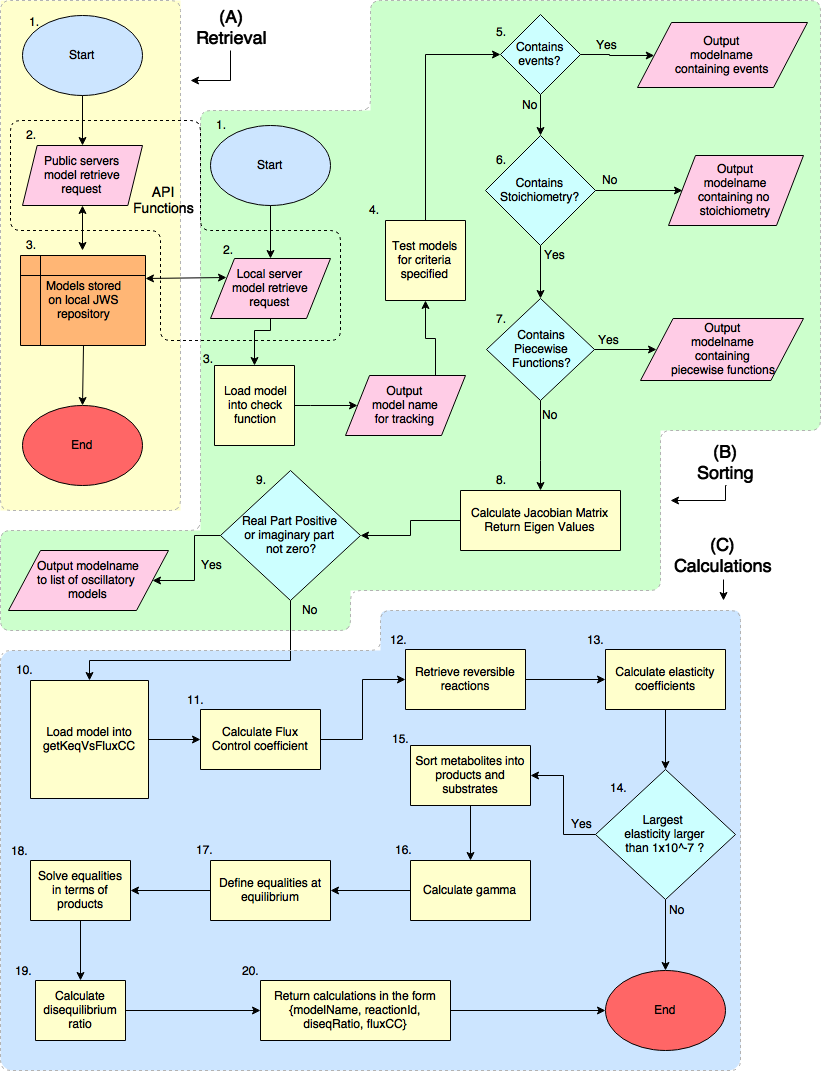
\includegraphics[width=1\textwidth]{Algorithm.png}
\centering
\caption{Overview diagram of algorithm indicating the flow of data throughout the run-time}
\label{fig:Algorithm}
\end{figure}

\section{Data processing} \label{Data processing}
Data processing refers to the act of information retrieval, conducted in a manner that is conducive to the transformation processes that will follow. With reference to figure \ref{dataFlow}, data processing entails the retrieval (A) and sorting (B) methods, as discussed in sections \ref{Retrieval} and \ref{Sorting}. For now however, the focus will be on the initial set up of the working environment used.

\section{Setting up the Working environment} \label{Working Environment}
The working environment was constructed in two parts, a data management component and a scripting language. The data management component is responsible for storing and translating model information, whilst the scripting language provides automation of compute operations required. These components were fulfilled by a local instance of \href{https://jjj.bio.vu.nl}{JWSOnline} and Mathematica v11 respectively. The JWSOnline server instance is hosted through the Docker platform, discussed in section \ref{Docker Installation}. For a more complete JWSOnline docker installation guide please refer to the documentation, available at \href{http://jws-docs.readthedocs.io/10_docker.html#building-the-jws-online-docker-image}.

\subsection{JWSOnline and Docker installation} \label{Docker Installation}
Docker, an open source platform, had the advantage of being platform agnostic. As such a Docker environment is self contained and easily reproducible, an advantage and requirement towards scientific inquiry. The main aim of a locally hosted \href{https://jjj.bio.vu.nl}{JWSOnline} server, was to achieve isolation from active production servers as to not inundate them with repetitive model upload, download, query and conversion operations. This proved especially useful considering the repetitive nature associated with a development and testing cycle for thousands of models. An added benefit was an observed increase in overall efficiency, taken as time to handle the entire data-set. This was due to internet connection speed and availability affecting only the initial retrieval of models from public servers. Overhead communication rates, between Mathematica and the server instance, was limited only by processor transfer rates. 

Starting out, the Docker host application is downloaded and installed for the operating system in question (OSX in this case) as instructed by the docker documentation available at \href{http://docker-sean.readthedocs.io}{http://docker-sean.readthedocs.io}. The JWSOnline Docker compose script, located at \href{http://jws-docs.readthedocs.io/10_docker.html#building-the-jws-online-docker-image} was copied and saved into a local file named "docker-compose.yml", noting the working directory. More information on the ".yml" format and the docker compose file in general can be obtained at \href{https://docs.docker.com/compose/compose-file/#compose-file-structure-and-examples} as a deeper description is outside of the scope of this thesis. 
Environment variables such as passwords and volume names in the "docker-compose.yml" is altered and saved to user specific requirements. This would be individual specific and other than the need for authentication the choice of these variables has no appreciable impact on further operations. Afterwards the images and services defined are retrieved by running the command "docker-compose pull" from within a terminal/bash environment (Please note this command must be performed from within the working directory noted earlier). The retrieved services are then launched by the "docker-compose up" command. This command starts the services as defined by the "docker-compose.yml" file. A successful installation and start up is confirmed by visiting the local host or loop back IP address (127.0.0.1) in a web browser and being greeted with a local JWSOnline homepage.

As mentioned earlier, the local JWSOnline installation provided the model handling portion of the working environment and as such needed to be able to communicate with the scripting language, Mathematica, at hand. The communications method native to JWSOnline, is in the form of a representational state transfer (REST) application program interface (API). As this is the basis of data transfer, the following section will provide a brief overview of example constructs, with specifics handled as applicable. 

\subsection{Communicating with JWSOnline via the \gls{rest} \gls{api}} \label{REST Communication}

The REST communications protocol allows applications and programs to share information with one another through a standardized method. A plethora of \gls{api} methods exist for various websites, but for the sake of simplicity the focus of this discussion will rest on the RESTFull web service framework \cite{rest2018}.

From a server perspective the \gls{rest} framework enables the control of access to internal application resources, while maintaining open access to services made available by such applications. These service endpoints are accessible to a client in the form of a basic URL request. This request uses the hypertext transfer protocol (HTTP) as is familiar from all generic web browsers. The REST framework was specifically developed in this way as to simplify the development process. Various applications can communicate with one another in a uniform manner \cite{rest2018}. Case and point, the availability of the \href{http://jjj.biochem.sun.ac.za}{JWSOnline} \gls{api} enabled the interaction of the web server with other applications or compute platforms, thus expanding the use of the application outside of the original project scope. 

HTTP requests can take on many forms, however for the purpose of this study the constructs will be fairly similar. For instance, one such example can take on the following form; \href{http://jjj.biochem.sun.ac.za/rest/models/teusink/mf}{http://jjj.biochem.sun.ac.za/rest/models/teusink/mf}. Various parts was interactively altered, as described in section \ref{Data processing}, in an attempt at an automated model handling algorithm. Let us therefore investigate and build upon this request. As is indicated by the "HTTP://" portion, this request utilizes the hypertext transport protocol (HTTP) at host address \href{jjj.biochem.sun.ac.za}{jjj.biochem.sun.ac.za}. The request is directed at the \gls{rest} endpoint within the "/models" directory to return the "/teusink" model in an "/mf" format. The returned result is a JSON data pair with model name and data contents as the first and second respective entries.

This example request above can be altered to return models based on specified criteria. For example, metabolic models can be returned by altering the request construct as follow; \href{http://jjj.biochem.sun.ac.za/rest/models/?id=&organism=&process=1&jwsmodel__model_type=}{\nolinkurl{http://jjj.biochem.sun.ac.za/rest/models/?id=\&organism=\&process=1\&jwsmodel\_\_model\_type=}}. In this request, "process=1" refers to models fulfilling the prerequisite of containing metabolic processes as defined by annotations from model creation and curation stages. A different one of these endpoints enabled the integration of models from an external source, to within the JWSOnline database. This proved useful in obtaining a larger sample size, as the \href{https://www.ebi.ac.uk/biomodels-main/}{BioModels} repository was consulted and integrated as described in section \ref{Data processing}. For more on JWSOnline specific REST endpoints, please refer to the JWSOnline documentation \cite{jwsdocs}. 


\subsection{Retrieval (A)} \label{Retrieval}
JWSOnline provides an endpoint for model retrieval from remote sources in the form of a restfull API. These The URL interaction functions of Mathematica, namely HTTPRequest and URLExecute, was used to construct a list of URLs linking to SBML models in both JWSOnline as well as Biomodels. The relevant parts of the example URL construct (\href{http://jjj.bio.vu.nl/rest/fetch/?type={type}&redirect={redirect}&remote={remote}}) was replaced by the remote URL's from the list created above. This command, initiated from the local JWSOnline instance, sequentially imported and converted each model to an internal data format. After which, these models were available for retrieval in any of the formats supported by JWSOnline. This raised the question of which model format would be best suited for the investigation at hand.

For the development of an automated algorithm, handling metabolic model analysis, a specific model format was needed. One that proved generic enough to facilitate the development of unattended automated functions, yet flexible enough to uniformly handle differences among models from various origins, destined for a diverse range of uses. As such five key aspects were identified as criteria for a suitable model format.

The model format had to: 
\begin{enumerate} \label{modelFormat}
  \item Consistently store similar data type at the same index - predictability
  \item Be easily understood by both humans and computers alike - ease of development
  \item Impart all of the information stored within the original model - consistency
  \item Keep information uniformly organized - accuracy
  \item Allow for direct computational interaction - accessibility
\end{enumerate}

\gls{sbml} provides a standardized structure to which biological models are kept. As such it seemed a logical first choice. However, although \gls{sbml} meets many of the requirements such as, predictability, accuracy and consistency, it does not meet all. This is due to the fact that \gls{sbml} makes complete sense to a computer, yet the syntax has a steep learning curve for the human eye. Combined with the fact that no native Mathematica \gls{sbml} parsing was supported at the time of development, the ease of development and accessibility aspects proved problematic. Therefore a method of model translation was called for. 

This translation process was achieved through the use of \href{https://jjj.bio.vu.nl}{JWSOnline}, whereby a \gls{sbml} model was retrieved from a remote server, converted and made available in matrix format (\gls{mf}) (One of the native JWSOnline data formats). In \gls{mf}, data is organized by content type. For example; rate-equations, metabolites, stoichiometry, parameter-sets and more are all grouped as nested lists, visually illustrated by figure \ref{fig:MatrixFormat}.  This format was chosen as it fulfilled all of the criteria as set out in list \ref{modelFormat}. It had the added advantage of enabling metabolic control calculations as discussed in section \ref{Calculations} to be done via matrix methods as described by \citeauthor{Hofmeyr2001}

Once a model has been handled by \href{https://jjj.bio.vu.nl}{JWSOnline},the end product of the translation process is made available as an \gls{api} endpoint allowing for the retrieval of the model. For example, the Teusink model can be found at \href{https://jjj.bio.vu.nl/rest/models/teusink/mf/}{https://jjj.bio.vu.nl/rest/models/teusink/mf/}. Additional resources to JWSOnline are available at \href{http://jws-docs.readthedocs.io/8_rest.html}{JWS Docs}. 

\begin{figure}[p]
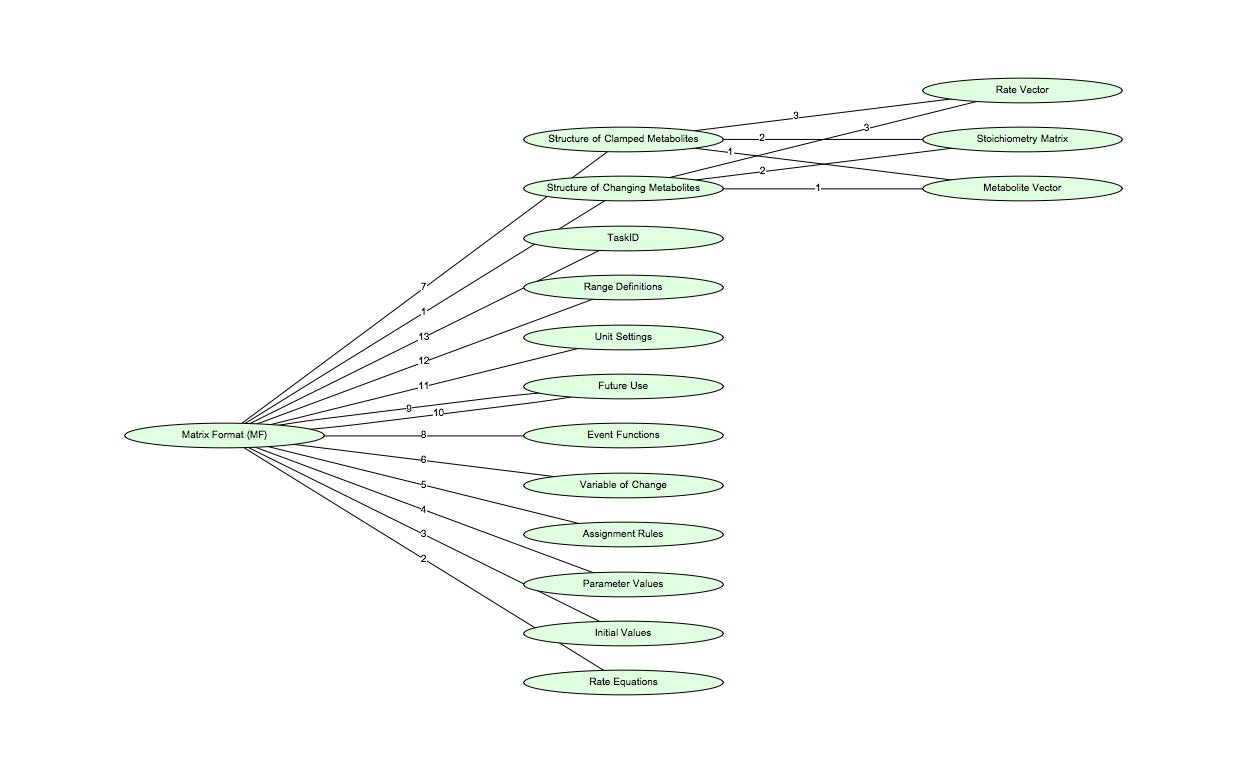
\includegraphics[width=1\textwidth]{MatrixFormat}
\centering
\caption{A graph representation of the Matrix Format (MF). Edge labels represent list index numbers and vertex labels denote content.}
\label{fig:MatrixFormat}
\end{figure}

\subsection{Sorting (B)}\label{Sorting}
Once all available models have been retrieved and stored within the local repository, the mf version was requested and returned as mentioned in section \ref{Retrieval}. These models then undergo a sorting and handling process, label B in figure \ref{fig:MatrixFormat}, in order to identify where models diverge from the main algorithm (3.). This process starts off by exporting the model name to a log file. Divergences in data flow was captured and visualized as discussed in chapter \ref{chp:4}. Vertices were defined as model and reaction names as well as endpoints specified. Edges in turn represented relationships and direction of procedural flow. Figure \ref{fig:MatrixFormat} was the end result of visualizing this log file and will be further discussed within section \ref{chp:4}. 

Once the initialization step was completed, a model was sent to a check function (4.). This function examines semantic structure as well as behaviour of models, in order to identify suitable models for the analysis at hand. The first process evaluates whether or not a model contains event functions. This is done by matching the pattern of an empty list to the appropriate sub list at index eight in the model (5.). A successful model is then checked for the presence of stoichiometry (6.). This is achieved by testing whether or not the stoichiometry list (index one) contains data. In other words, when the length of the list at the stoichiometry index is equal to zero, the model contains no stoichiometry and is handled and logged as such. Model event triggers, of the kind described above, can also be specified in terms of piece-wise functions (7.). As no a priori knowledge on the timing or the effect of these event triggers upon the steady state and control behaviour were available, they were also identified and logged. This identification was done based on the pattern of a reaction containing the string "Piecewise" as the function is referred to. 

These steps served as a minimal-validation for initial models. The order of operation proved important, as these procedures were not as computationally intensive as simulation and calculation operations. Therefore computational efficiency was gained in optimizing the order of operations. 

Following the semantic and structural tests described above, the stability of a model had to be assessed. This was done by evaluating model steady state behaviour. For this purpose the Jacobian matrix was consulted (8.). As is known from linear algebra, the eigenvalues of a Jacobian matrix holds information on the stability of a system of ODE's. The system is said to converge to a stable state when a decrease in perturbation is observed, in other words, from the jacobian matrix, real parts of eigenvalues are negative pointing to a decrease in initial perturbations. In contrast a positive eigenvalue points to a divergence from a stable state, as a perturbation is amplified. A third condition was the occurrence of a positive eigenvalue with a non zero imaginary part. These results are indicative of a system oscillating around some state, be it stable or unstable periodic behaviour. As such, model names exhibiting oscillatory behaviour were identified and written to our log file. For a simple test of stability, a Jacobian matrix that is invertible could serve as a positive test of steady-state \cite{Hofmeyr2001}.  

A model that have reached this point in the algorithm marked a checkpoint and was written, in full mf format, to a text file for record and future uses. Next up the model was sent for the simulation and calculation procedures as is described in the following section and as can be seen in figure \ref{dataFlow} number ten.


Biological model analysis platforms range from stand-alone applications, the likes of Jarnac, COPASI, CellDesigner and BioNetGen, to  add-on modules and libraries such as LibRoadRunner, COBRA, Pysces, SimBiology and Simulink, for the Python and Matlab scripting languages respectively \cite{Sauro2000, Hoops2006, Olivier2005, Somogyi2015, Harris2016, Laurent2017}. JWSOnline is a web based interactive interface for model creation, curation and simulation. A task achieved by utilizing custom Mathematica model manipulation packages alongside a combination of the above mentioned add-on modules, as described by \cite{Olivier2004, jwsdocs}. The JWSOnline platform is specifically mentioned here as it will form as a basis of tools, as described in section \ref{Working Environment} and \ref{Data processing}. 

The tools mentioned above, along with protocols and endpoints discussed in \ref{Working Environment}, prove useful in single isolated instances. However, when paired with scripting languages they can become immensely powerful and endlessly more useful. This is because automated computational operations can be performed faster, more accurately and for longer periods of time than would be otherwise possible by human minds. The following section is therefore dedicated to the introduction and explanation of individual steps, leading up to the entirety of such an automated model interrogation algorithm responsible for the collection of data utilized in the analysis, described in section \ref{Analysis}. 










\subsection{Calculations (C)} \label{Calculations}
The \gls{steady-state} of a model was calculated and the flux control coefficients were determined (10.). This was done utilizing linear algebra methods as described by \citeauthor{Hofmeyr2001}. This method entails the reduction of a stoichiometry matrix $N$ to row echelon form by Gaussian elimination. The reduced matrix $N_R$ contains the independent reactions and can be returned to $N$ matrix by defining a link matrix $L$ such that $N = LN_R$. Further information on the dependent and independent relationships are possible, yet will not be discussed here. 

Elasticity co\"efficients $\Bar{\mathcal{E}}$ were determined by taking the partial derivatives of reaction rates with respect to steady state concentrations. This notation stems from the article by \citeauthor{Hofmeyr2001} with the bar on $\mathcal{E}$ indicating unscaled elasticities. Scaling can be applied in order to generate dimensionless elasticities $\mathcal{E}$. As mentioned earlier, the steady state is influenced by parameters populated from experimental procedures and as such, each steady-state is unique to parameter values and initial conditions. 

A steady-state consists of metabolite concentrations $s$ as well as flux through values $J$. Changes to these steady-state values $(s,J)$, due to perturbations of parameter $p$, can be approximated by the following means. For metabolite concentrations $s_2 = s_1 + \frac{\partial s}{\partial p}(p_2 - p_1)$ and fluxes $J_2 = J_1 + \frac{\partial J}{\partial p}(p_2 - p_1)$. 

From the above matrices, the flux control co\"efficients were determined. The product of $N_R\Bar{\mathcal{E}}L$ being defined as the Jacobian matrix $M$. Further discussions on the Jacobian matrix will follow. For now however the importance lies in the calculation of concentration control co\"efficients towards the end of determining flux control co\"efficients.

The concentration control co\"efficients indicate a measurement of, as the name suggests, relative changes to metabolite concentrations $s$ brought about by parameter perturbations $p$. From the matrix formalism the concentration control co\"efficients $\Bar{C^s}$ can be determined from the link matrix $L$ the Jacobian matrix $M$ and the reduced stoichometry matrix $N_R$ as $\Bar{C^s}=-LM^{-1}N_R$. Flux control co\"efficients were then calculated via the following equation $\Bar{C}^J = \Bar{\mathcal{E}_s}\Bar{C^s}+ I_n$ \cite{Hofmeyr2001}.

From the above, many results were generated and as such filtering and sorting proceeded with models containing negative flux control coefficients upon themselves. A perturbation, towards flux control co\"efficient determination, is considered as an increase or decrease in enzyme activity or concentration. Therefore a negative flux control was deemed improbable, as an increase in enzyme concentration would logically not lead to a decrease in reaction rate. No further investigation into this was committed as this is outside the scope of this thesis.

Considering that disequilibrium ratio calculations are only applicable within reactions proceeding in a reversible manner, a test function was developed to identified these reactions. A reversible reaction was defined as a rate equation containing a negative part within the numerator portion. This was drawn from general reaction rates where $v_{net} = v_{forward} - v_{reverse}$ thus allowing a rate to become negative (reversible) under appropriate conditions. The numerator is therefore recast into base components and tested for the presence of a negative-one term (12.). This was achieved by utilizing the tree form structures available to Mathematica leading to an equation expanded to smallest component parts. The position of these reversible reactions were then stored in a variable for use in disequilibrium calculations later. 

As can be seen from the calculations of flux control co\"efficients prior, an inverse of the Jacobian matrix is calculated (13.) \citeauthor{Hofmeyr2001}. Therefore, as the Jacobian approaches zero, an inverse would approach infinity. This introduced errors due to machine precision digit and accuracy limitations when elasticity values were too small. As such a further step in ensuring model validity was implemented via elasticity calculation checks. Maximum elasticity values of the system were compared to a threshold, chosen as $1 \cdot 10^{-10}$. The choice of this threshold was based on observation of failed calculations from models in a "trial and error manner".  Models surpassing this threshold was passed to the following step (14.). 

To calculate disequilibrium ratios, knowledge of metabolite identity (substrate/product) was needed. Metabolites were identified through the use of the stoichiometry matrix. One can extract products and substrates on the basis of stoichiometry values that are larger or smaller than zero respectively(15.). Returning a reaction id linked to product id allowed for the consistent handling of applicable reactions. In the case of multiple products only the first product was returned for use, more were not required. Once products have been identified, gamma was determined by raising each metabolite in a reaction to the power of it's corresponding stoichiometry, leading to the first part of symbolic gamma construction. From vector 
\[
S
=
\begin{bmatrix}
    s_{1} \\
    s_{2} \\
    s_{3} \\
    \vdots \\
    s_{n} 
\end{bmatrix}
\]

each component is raised to the corresponding collumn value from

\[
N 
=
\begin{bmatrix}
    x_{11} & x_{12} & x_{13} & \dots  & x_{1n} \\
    x_{21} & x_{22} & x_{23} & \dots  & x_{2n} \\
    \vdots & \vdots & \vdots & \ddots & \vdots \\
    x_{d1} & x_{d2} & x_{d3} & \dots  & x_{dn}
\end{bmatrix}
\]

leading to 

\[
S^N
=
\begin{bmatrix}
    s_1^{x_{11}} & s_2^{x_{12}} & s_3^{x_{13}} & \dots  & s_n^{x_{1n}} \\
    s_1^{x_{21}} & s_2^{x_{22}} & s_3^{x_{23}} & \dots  & s_n^{x_{2n}} \\
    \vdots & \vdots & \vdots & \ddots & \vdots \\
    s_1^{x_{d1}} & s_2^{x_{d2}} & s_3^{x_{d3}} & \dots  & s_n^{x_{dn}}
\end{bmatrix}
\]


For the second part, each of these exponents were multiplied by one another according to the respective reaction rows 

\[
V
=
\begin{bmatrix}
    V_{1} \\
    V_{2} \\
    \vdots \\
    V_{d} 
\end{bmatrix}
\]

such that

\[
\gamma 
=
\begin{bmatrix}
    s_1^{x_{11}}s_2^{x_{12}}s_3^{x_{13}} \dots s_n^{x_{1n}} \\
    s_1^{x_{21}}s_2^{x_{22}}s_3^{x_{23}} \dots s_n^{x_{2n}} \\
    \vdots\\
    s_1^{x_{d1}}s_2^{x_{d2}}s_3^{x_{d3}}\dots s_n^{x_{dn}}
\end{bmatrix}
\]

From the above it can be seen that stoichiometries of zero will result in power calculations of one. With negative and positive stoichiometries as denominators and numerators respectively, resulting in the gamma fraction \gamma of the specific reaction. $K_{eq}$ calculations where done, as an example from the Tuesink model mention earlier. The 2-Phospho-D-glycerate 2,3-phosphomutase catalyzed reaction leading from P2G to PEP is used as an example, where an equality is defined in terms of equilibrium, \textit{i.e.} the rate equation $v_n$ equals zero.

\begin{equation}
v = \frac{V_mENO([P2G] - \frac{[PEP]}{K_{eq}ENO})}{K_mENOP2G(1 + \frac{[P2G]}{K_mENOP2G} + \frac{[PEP]}{K_mENOPEP})} = 0
\end{equation}

Following this, the equality was symbolically solved in terms of the product identified in (15.). In the example case PEP is the product. As such the above equation in terms of PEP becomes

\begin{equation}\label{PEP}
PEP = K_{eq}ENOP2G
\end{equation}

From the calculations above, this reaction has

\begin{equation}\label{gamma}
\gamma=\frac{[PEP]^1}{[P2G]^1}
\end{equation}

Substitution of equation \ref{PEP} into \ref{gamma} yields $\gamma$ at equilibrium, otherwise known as $K_{eq}$. Therefore

\begin{equation}\label{Keq}
K_{eq}=K_{eq}ENO
\end{equation}

Taking equation \ref{gamma} divided by \ref{Keq} gives us the disequilibrium ratio
\begin{equation}
\rho = \frac{\gamma}{K_{eq}} = \frac{\frac{[PEP]^1}{[P2G]^1}}{K_{eq}ENO}
\end{equation}

Substituting steady-state values allows for the calculation of the numerical disequilibrium ratio. This was the generic manner in which disequilibrium calculations were done. From this methods described, two values were returned per reaction. The flux control co\"efficient as well as the disequilibrium ratio. These results were used further towards the analysis at hand.

\section{Analysis} \label{Analysis}

\chapter{Results and Discussion} \label{chp:4}

The methods of this investigation, as described in chapter \ref{chp:3}, lead to the generation of a directed graph, generated from the log file, indicating the flow of model information as can be seen in figure \ref{Graph_modDistro}. 

\begin{figure}[p] \label{Graph_modDistro}
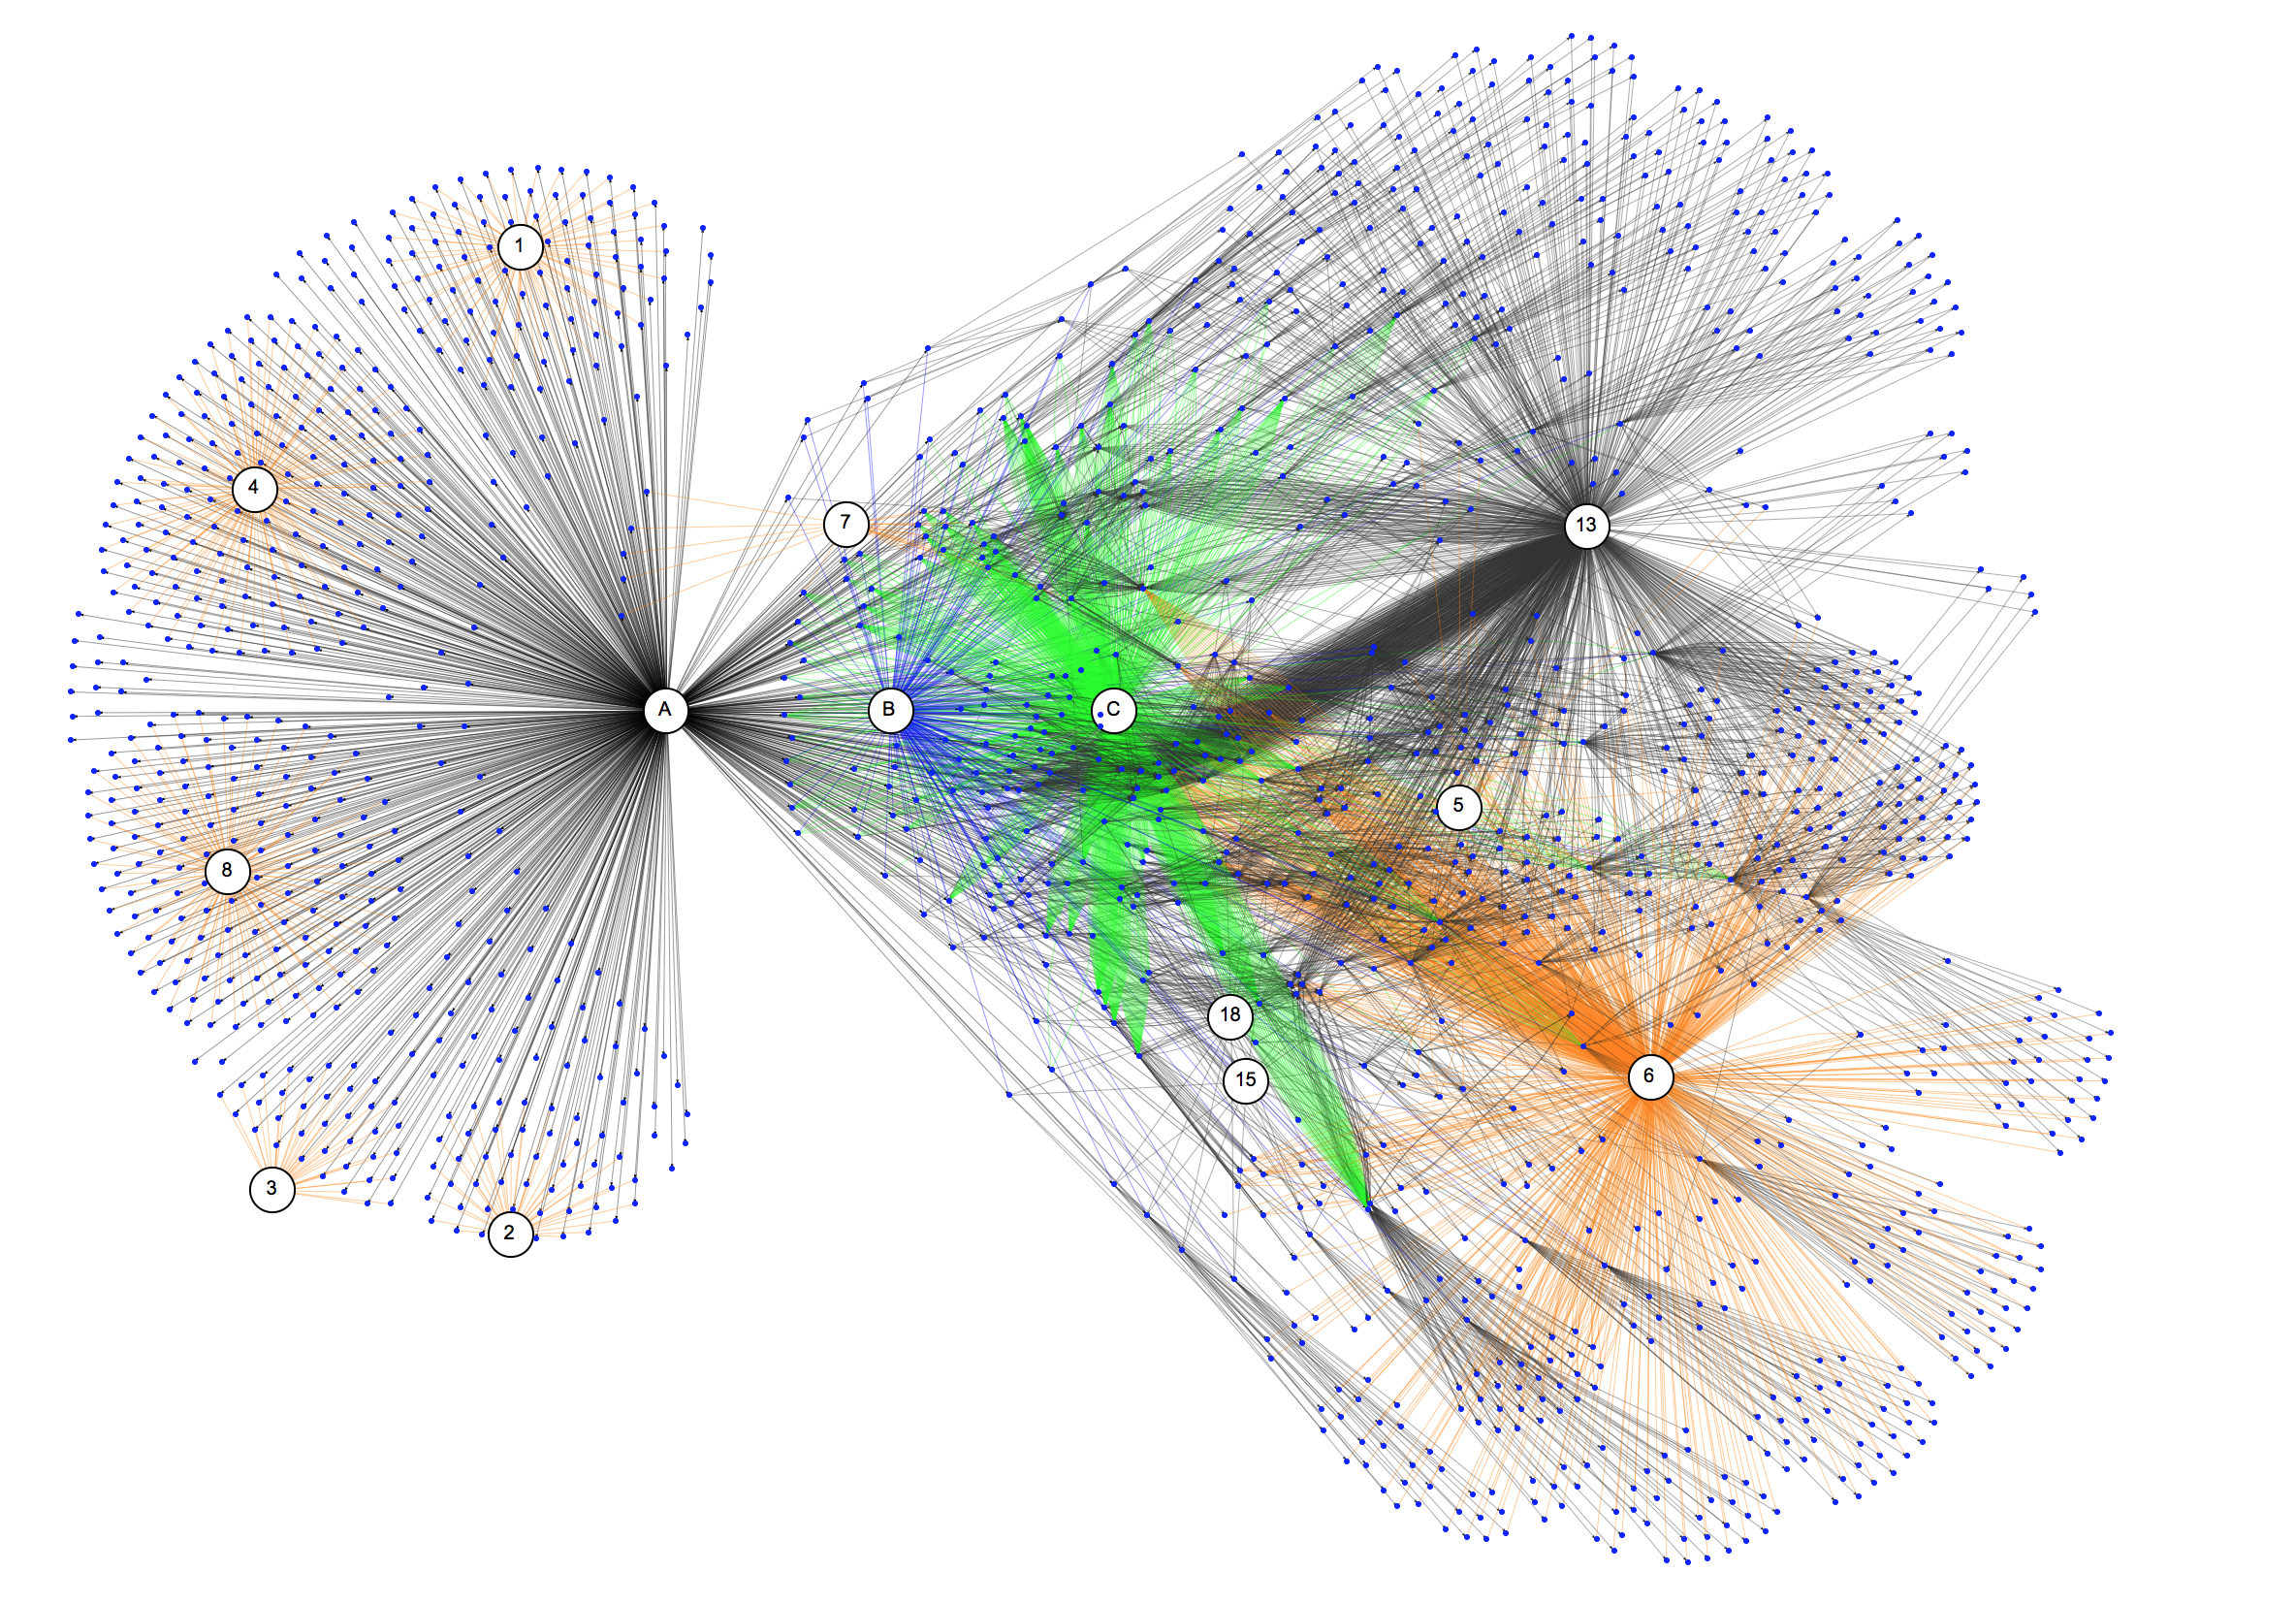
\includegraphics[width=1\textwidth]{figs/Digraph.png}
\centering
\caption{Directed graph indicating the flow of models as they are filtered by the algorithm described in chapter \ref{chp:3}. 
Important checkpoints are indicated by letters, with $A \rightarrow{}$ All models, $B \rightarrow{}$ Has reversible rates and $C \rightarrow{}$ Initial check functions passed. Filter criteria is labeled by number, with $1 \rightarrow{}$ No stoichiometries, $2 \rightarrow{}$ Events, $3 \rightarrow{}$ Piece-wise, $4 \rightarrow{}$ Oscillatory, $5 \rightarrow{}$ Division by zero, $6 \rightarrow{}$ Flux summation error, $7 \rightarrow{}$ Timed out, $8 \rightarrow{}$ No reversible reactions, $9 \rightarrow{}$ Import error, $10 \rightarrow{}$ Negative FCC, $11 \rightarrow{}$ Steady-state error, $12 \rightarrow{}$ Division by zero, $13 \rightarrow{}$ No product or substrate, $14 \rightarrow{}$ Replacement errors, $15 \rightarrow{}$ Small maximum elasticity coefficient, $16 \rightarrow{}$ No reversible reactions, $17 \rightarrow{}$ Flux calculation error and $18 \rightarrow{}$ No flux results generated.}
\end{figure}

This figure allows one to gain an overview of the model space. The models of importance were ones leading towards $c$ with green line, it is however clear that many models did not meet the requirements, $86\%$ to be exact. The final data contains reactions from 111 models, yielding 843 data points on disequilibrium ratio and flux control co\"efficient. The probability distributions of this data can be seen in figure \ref{TwoResPDF}.

A probability density function of the distribution, normalized via Gaussian kernel, was visualized by a contour plot. This plot can be seen at two resolutions in figure \ref{TwoResPDF}. It is clear that there exists a tendency for reactions close to equilibrium to not have a large degree of own flux control. As can be seen from figure \ref{TwoResPDF} $a$, there is no representative reaction with a control co\"eficient larger than $0.4$. On the opposite side of the scale it is observed that reactions with a larger than $0.4$ control co\"efficient reside within the region of $\rho < 0.1$. At a higher resolution however, figure \ref{TwoResPDF} $b$ indicates that reactions close to equilibrium ($\rho > 0.9$), with larger than $0.4$ flux control co\"efficients  do exist, albeit few. The \rho separation values chosen above, can be seen in figure \ref{PredictionConfidence}. These values echo the conclusion by \citeauthor{Rohwer2009} as discussed in chapter \ref{chp:2}.

To gain some degree of confidence in the visual findings, the data was utilized in the training of three separate neural networks. The probability density functions of the predicted flux control co\"efficients were visualised on the same axes as can be seen in figure \ref{PredConf}

\begin{figure}[p] \label{TwoResPDF}
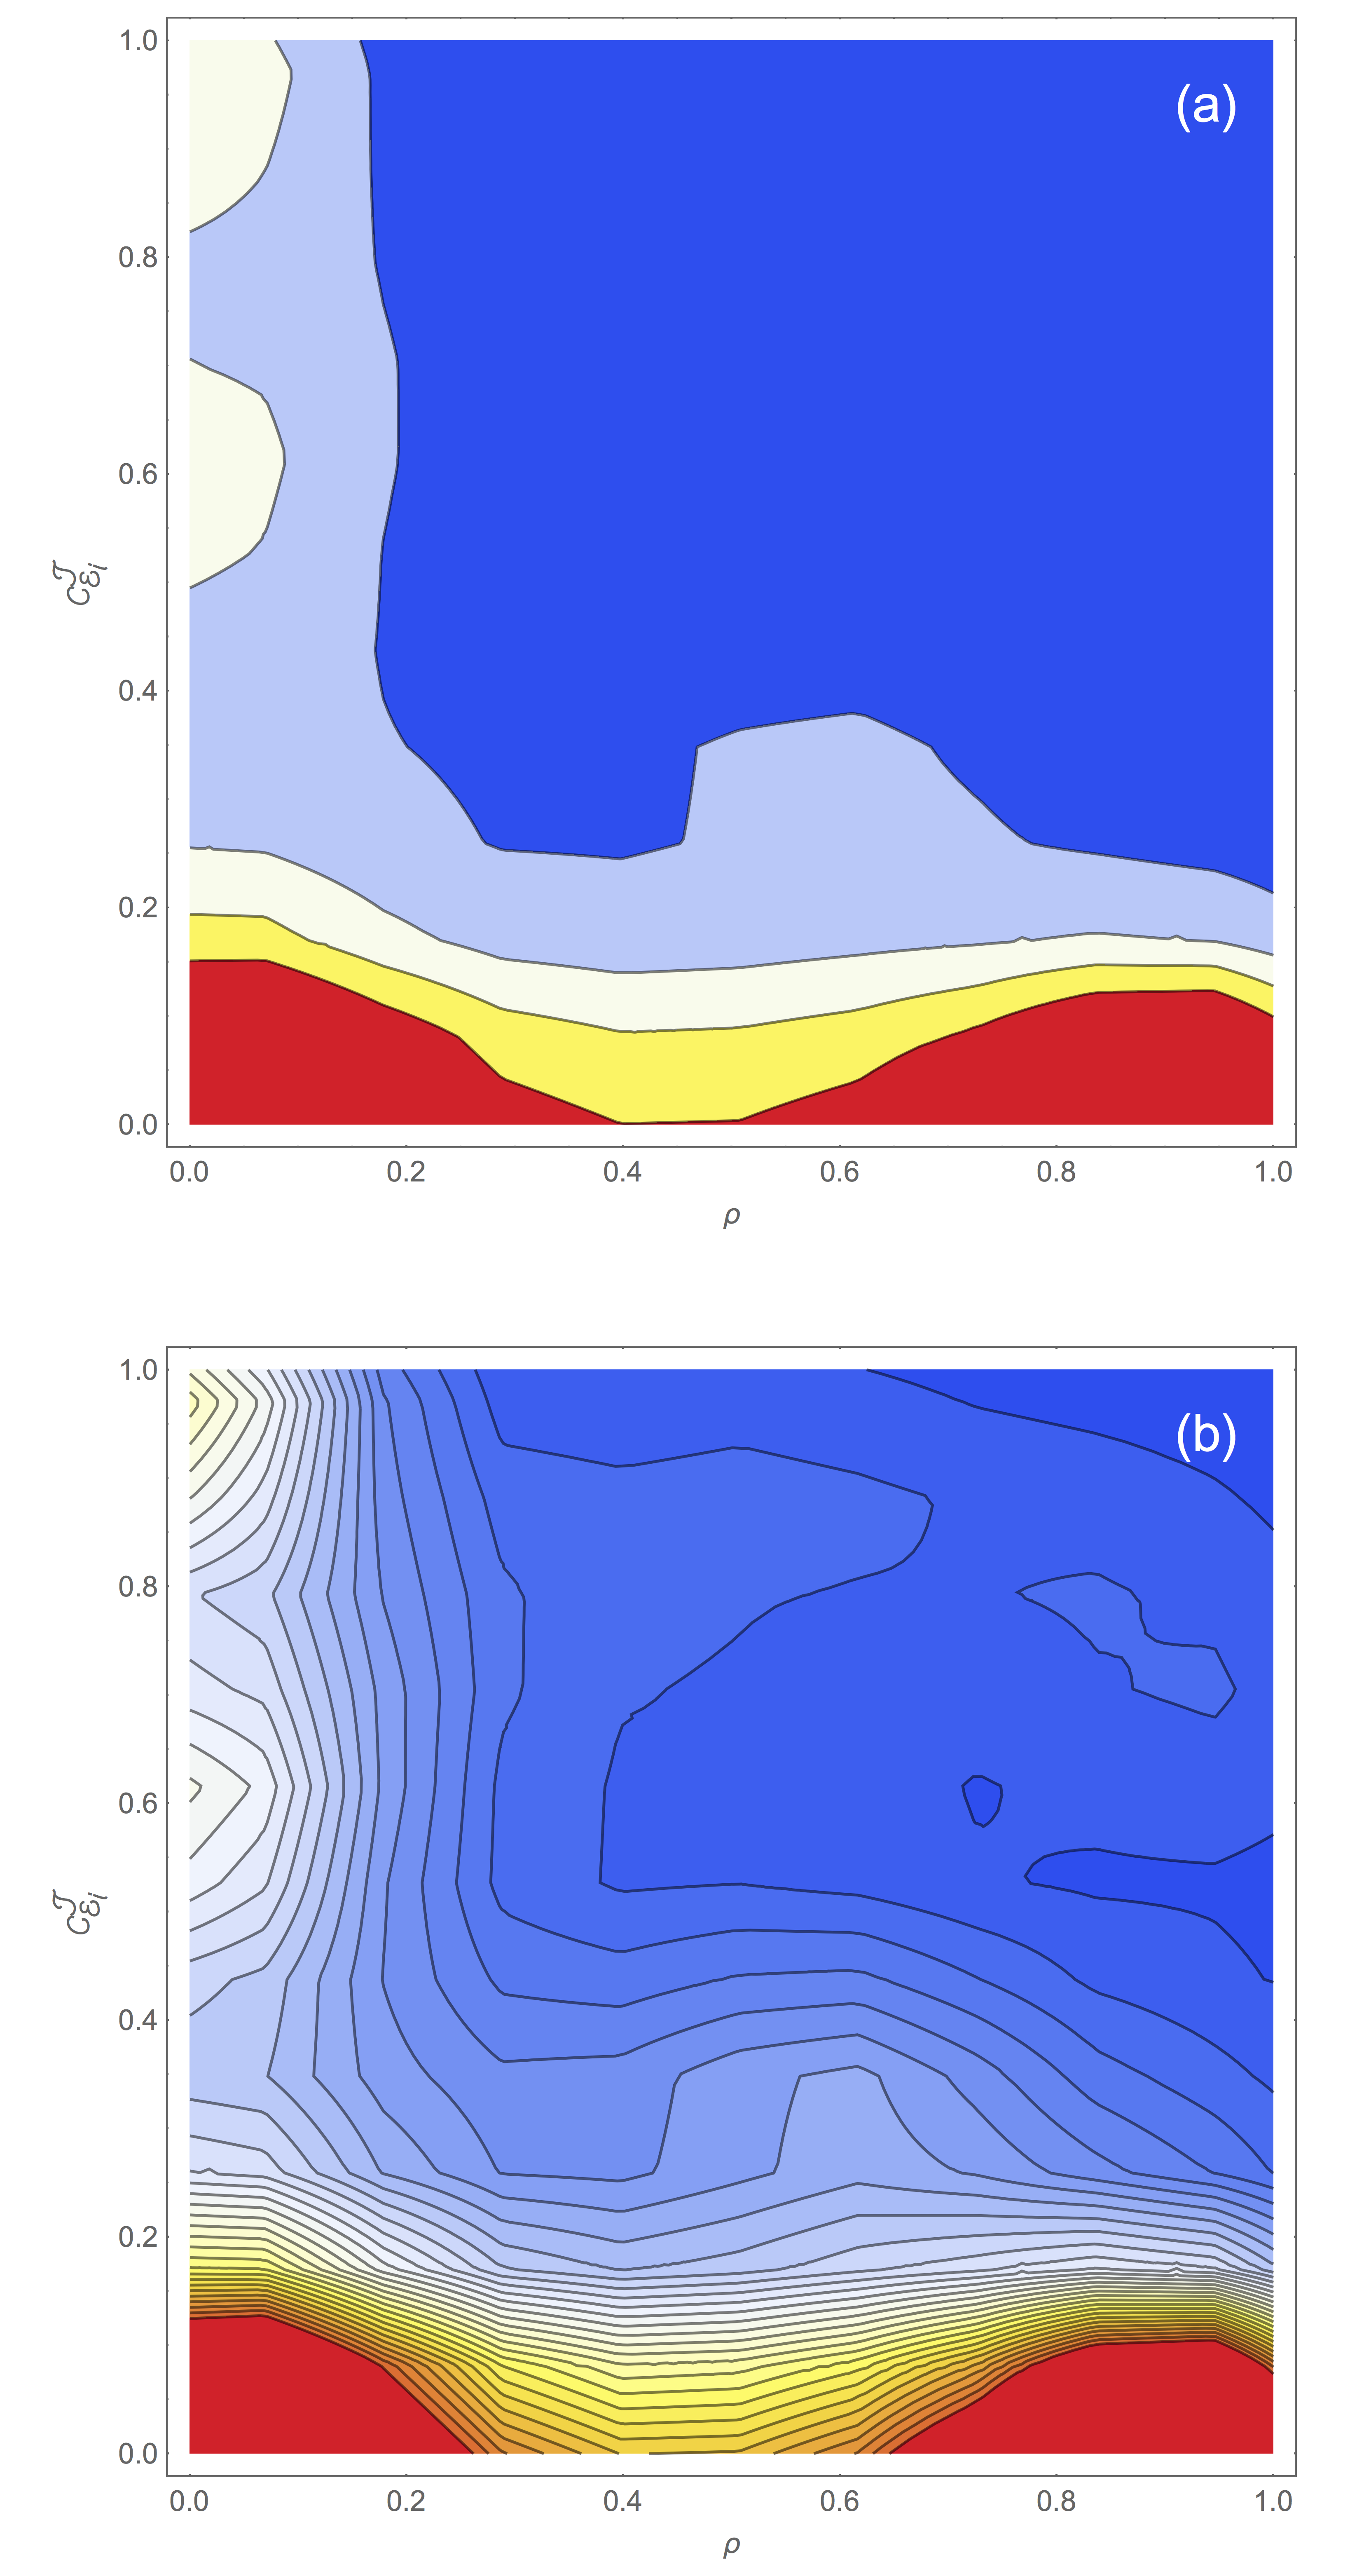
\includegraphics[width=0.8\textwidth]{figs/TwoResPDF.png}
\centering
\caption{Two resolutions was obtained by varying the contour amount visualized, $a = 4$ and $b = 30$, from the probability density function calculated in chapter \ref{chp:3}. This data is on the disequilibrium ratio ($\rho$) and the own flux control coefficient ($C_{E_i}^J$), normalized to the probability space of one. Red and blue respectively denote high and low density areas of data points.}
\end{figure}

\begin{figure}[p] 
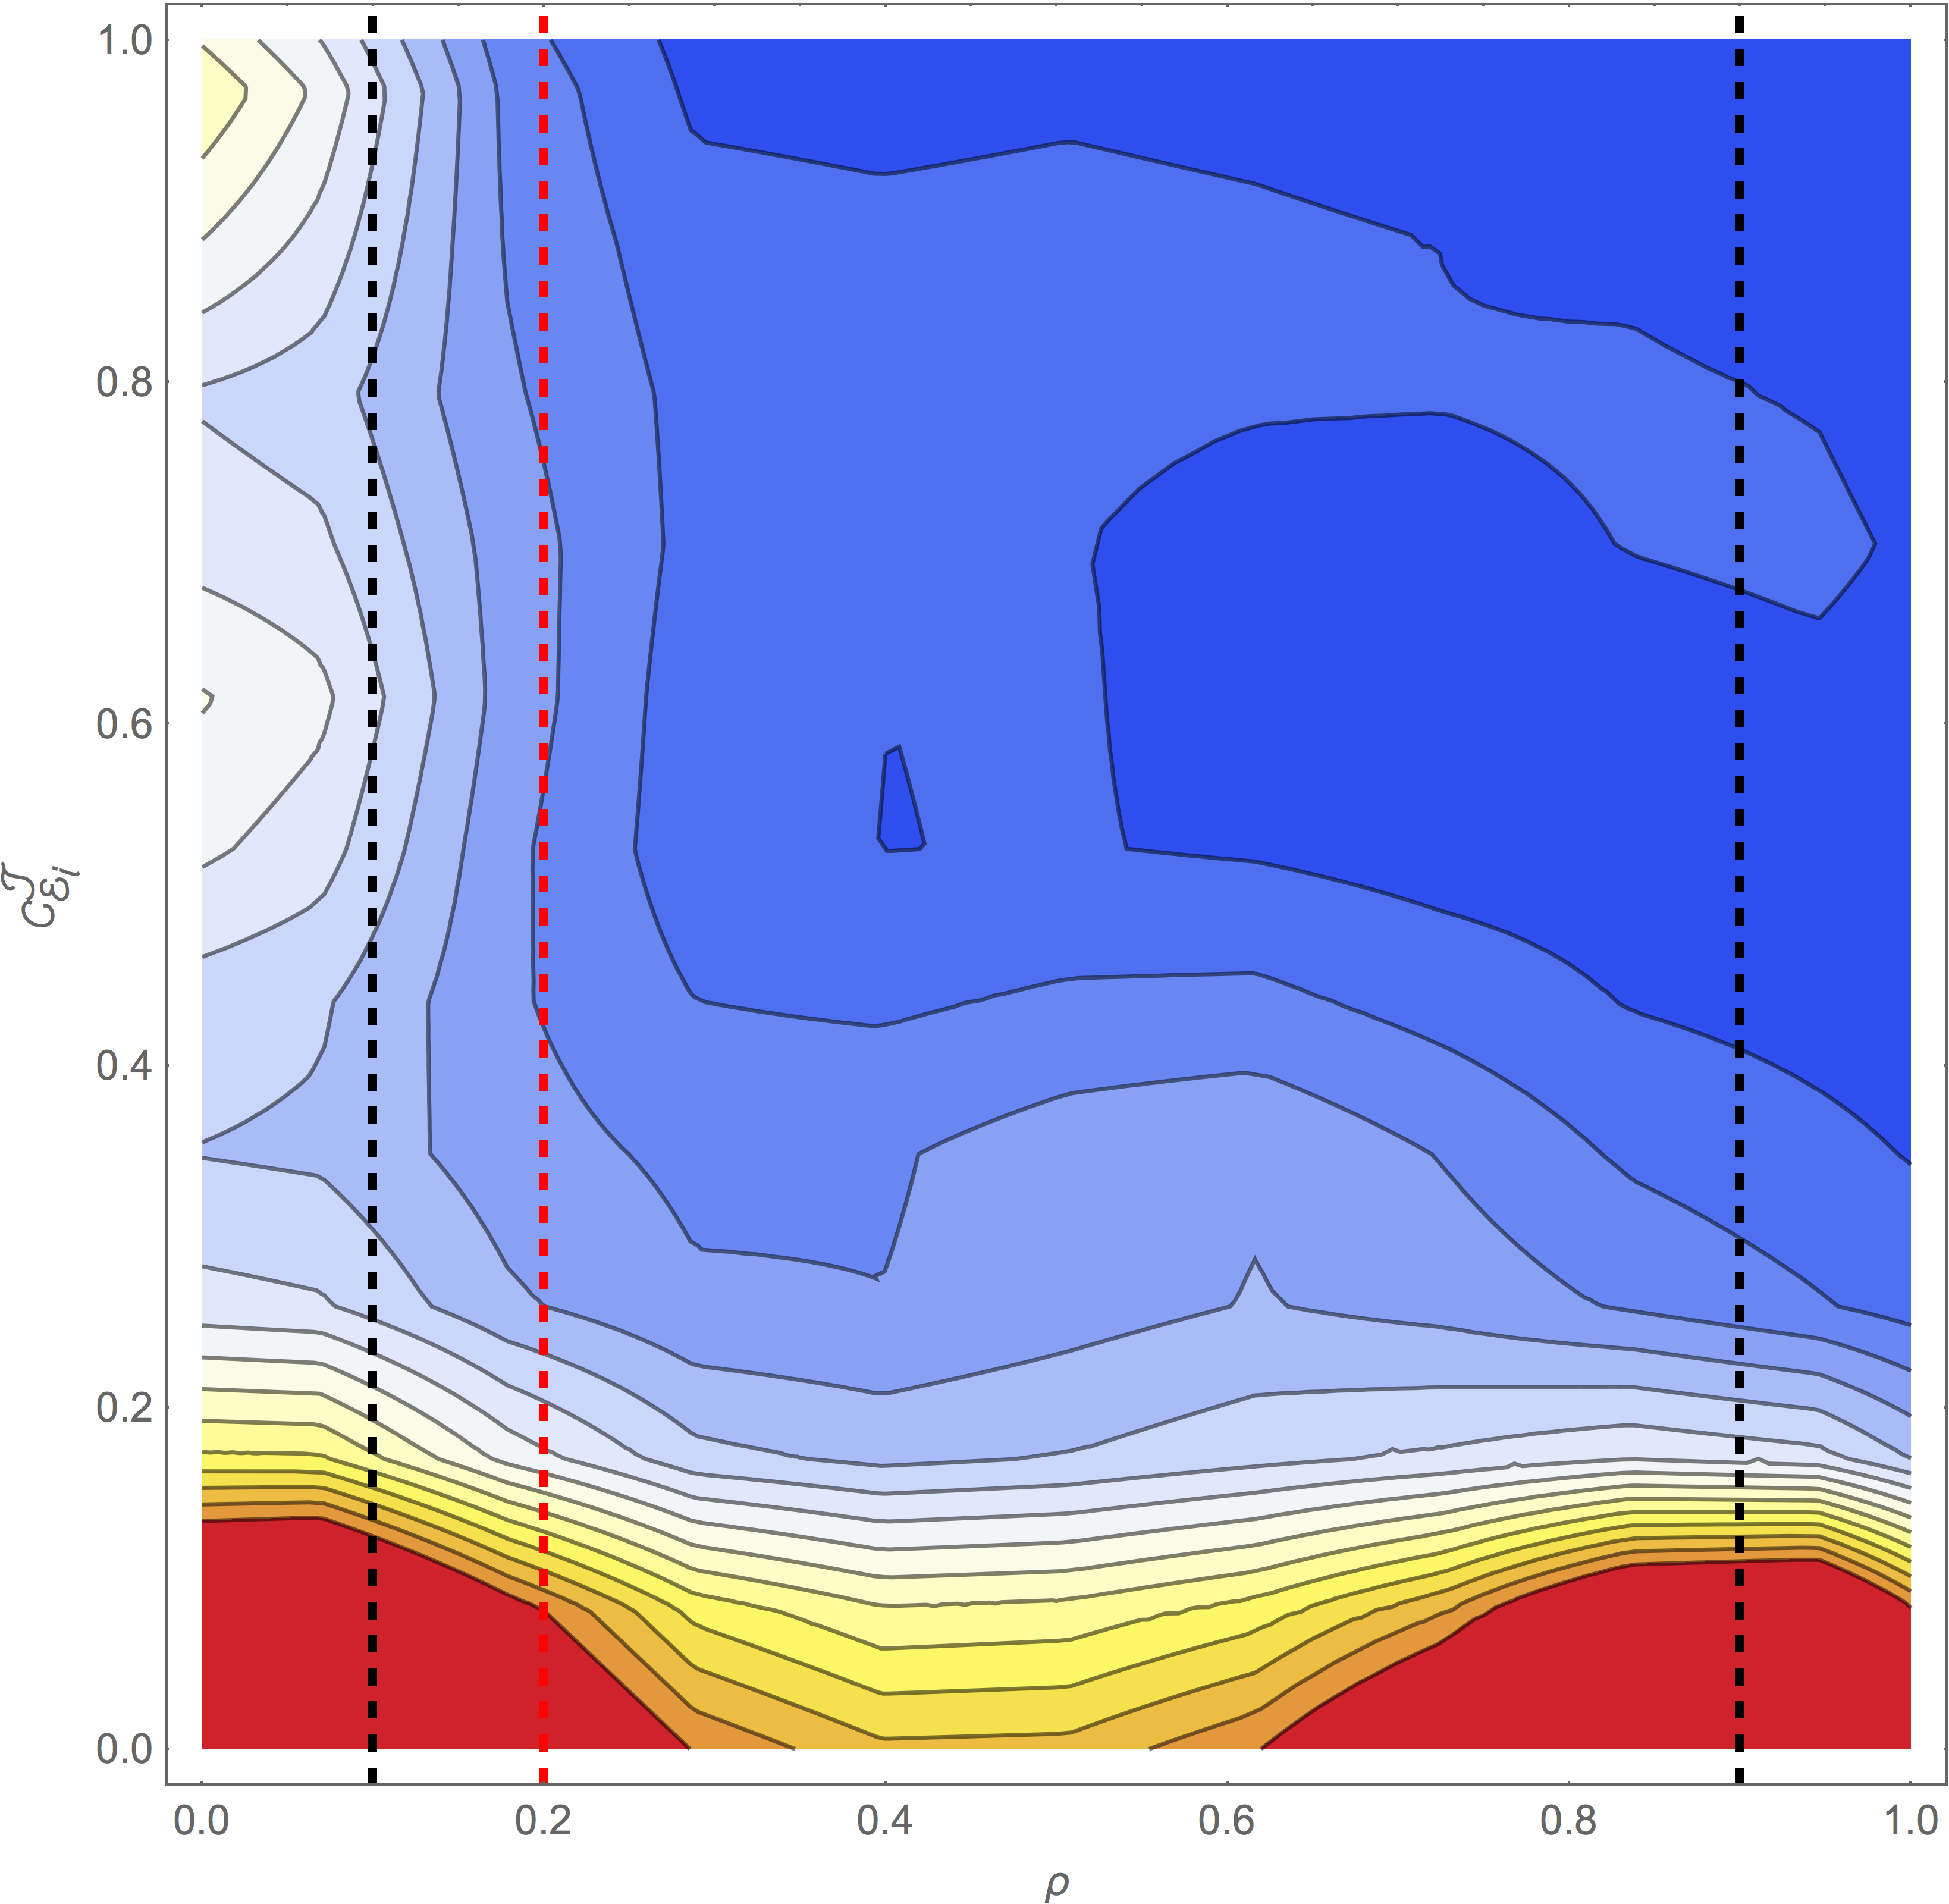
\includegraphics[width=0.8\textwidth]{figs/LitCompare.png} \label{LitCompare}
\centering
\caption{Probability density function of data gathered. This data is on the disequilibrium ratio ($\rho$) and the own flux control coefficient ($C_{E_i}^J$), normalized to the probability space of 1. Red and blue respectively denote high and low density areas of data points. The black (\citeauthor{Rohwer2009}) and red (\citeauthor{ROLLESTON1972}) dashed lines indicate respective authors views, as referred to in chapter \ref{chp:2}, on probable conditions of dominating contributions to regulation.}

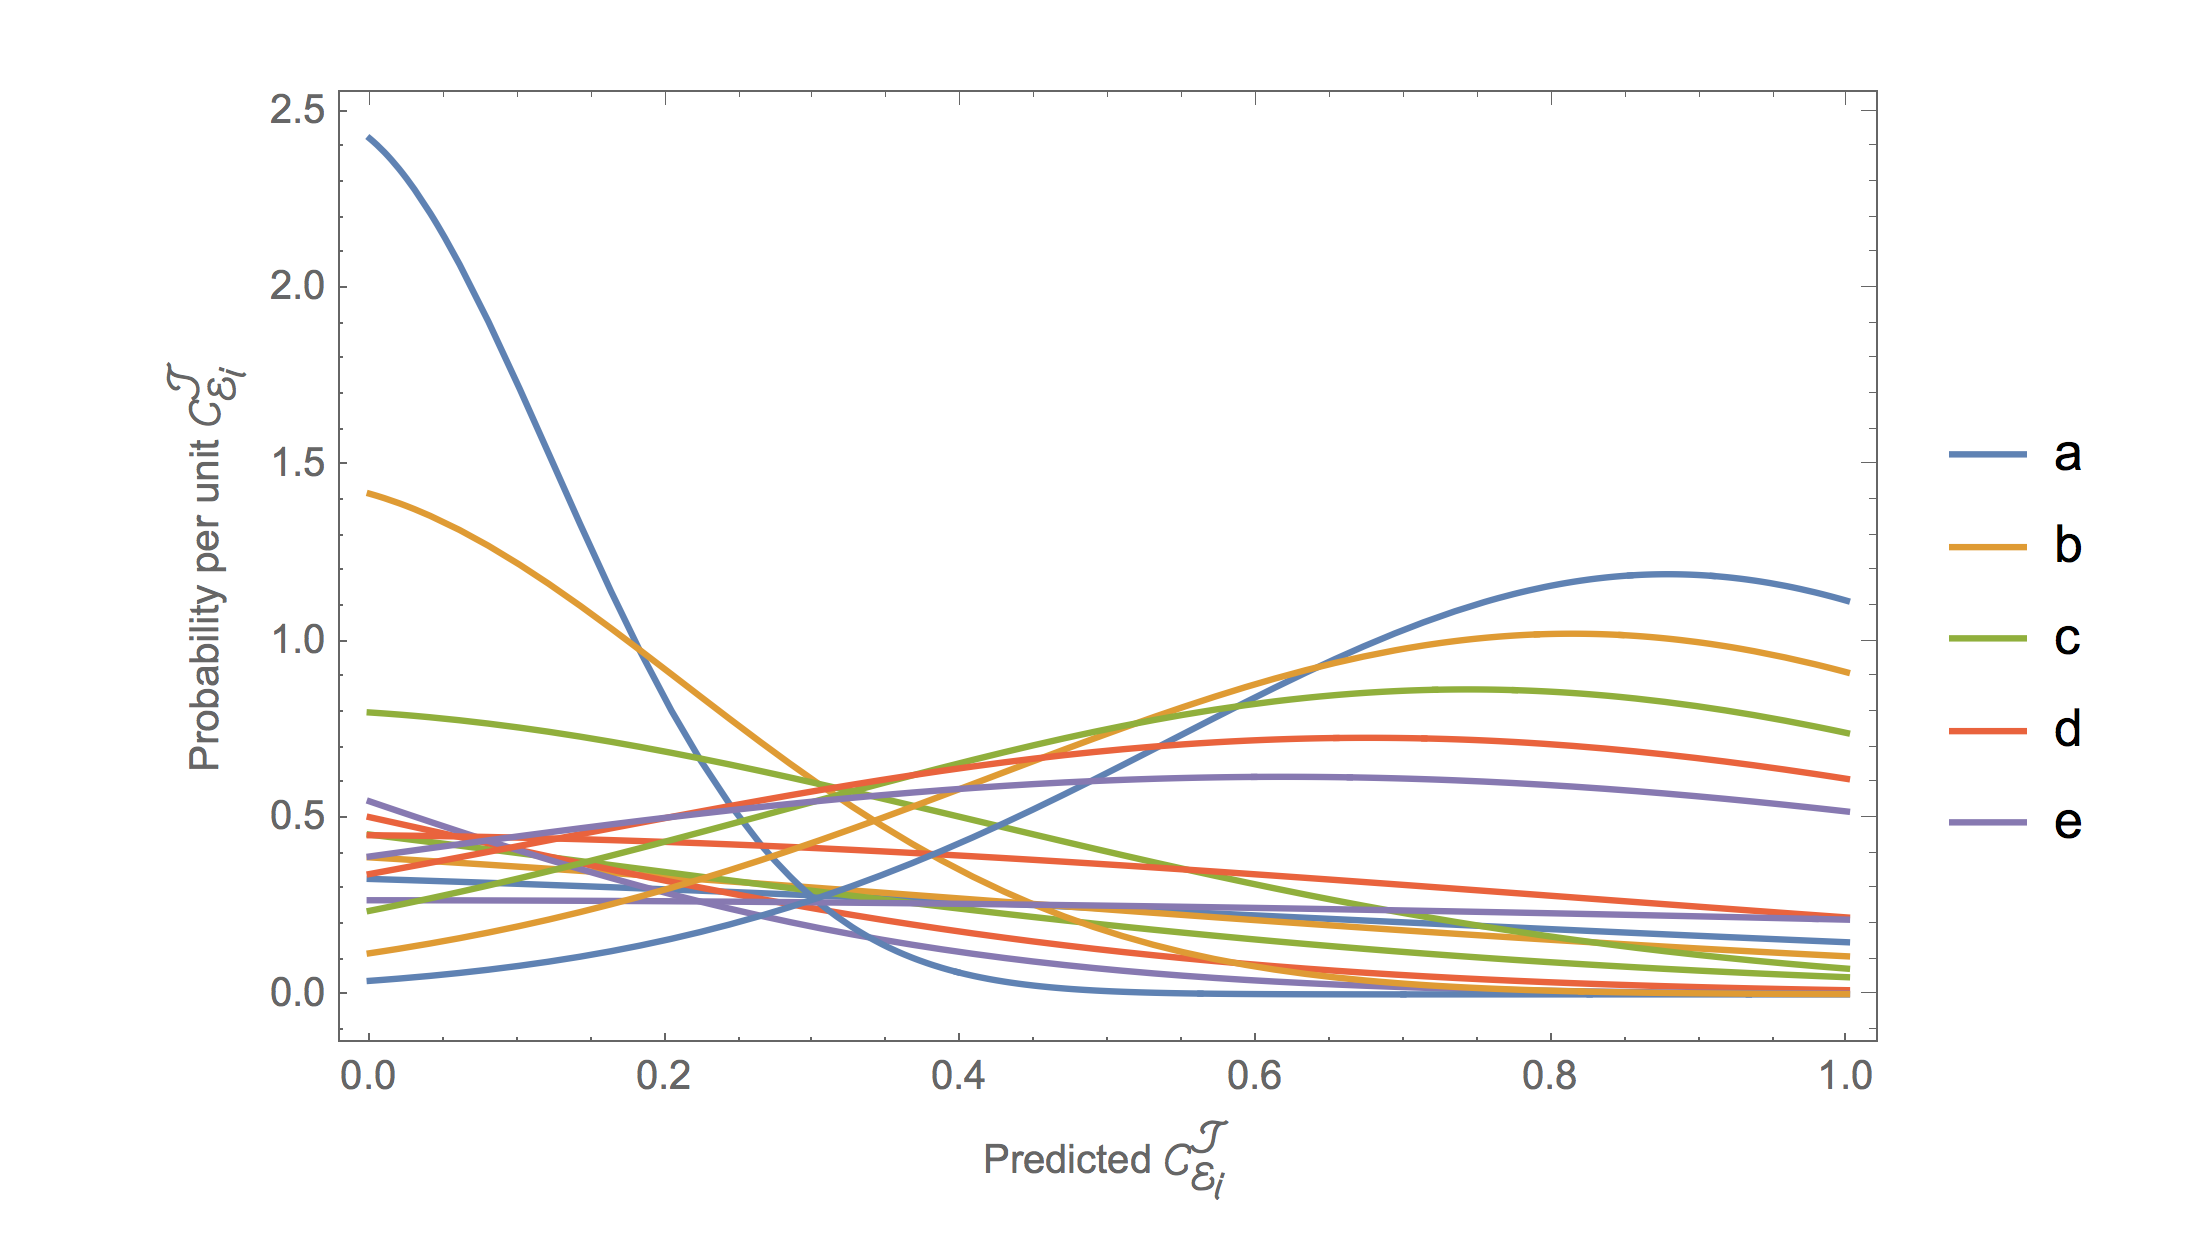
\includegraphics[width=1\textwidth]{figs/PredConf.png} \label{PredictionConfidence}
\centering
\caption{Probability density functions of estimates on flux control co\"efficients. Predictions were made at six disequilibrium ratio values, from three respective Mathematica neural network predictor functions, as referred to in \ref{chp:3}. The chosen disequilibrium ratios were $a = 0.01$, $b = 0.25$, $c = 0.50$, $d = 0.75$, and $e = 0.99$ respectively.}
\end{figure}


Four hypothesis were set in order to further evaluate the gathered data. Based on the premise of covering all possible combinations of variables the first of these postulates that; large flux control co\"efficients are witnessed at small disequilibrium ratios.

\begin{equation}
    \rho \ll 1 \Longrightarrow C_{E_i}^J \gg 0
\end{equation}

The second is derived from the reciprocal supposition, where large flux control co\"efficients necessarily relates to small disequilibrium ratios.

\begin{equation}
    C_{E_i}^J \gg 0 \Longrightarrow \rho \ll 1
\end{equation}

With the first two hypothesis relating distances far from equilibrium to control, the third and forth relates to the opposite. With disequilibrium ratios approaching unity, the third hypothesis necessitates a small observed flux control co\"efficient.

\begin{equation}
    \rho \approx 1 \Longrightarrow C_{E_i}^J \ll 1
\end{equation}

While the final hypothesis views disequilibrium ratios as necessarily approaching unity where small flux control co\"efficients are concerned.

\begin{equation}
    C_{E_i}^J \ll 1 \Longrightarrow \rho \approx 1
\end{equation}

Applying these four hypothesis to the probability density function obtained from the data, one can gain insights into how thermodynamic states influence control behaviour. 





%==== Appendices ====================================================
\appendix
\appendixpage\relax

%\include{contents/App-1}
%\include{contents/App-2}
%\include{contents/App-3}

%==== Bibliography acro's & Index ===================================
\backmatter

\bibliography{backmatter/lit_review}

\end{document}
